\documentclass[12pt, a4paper]{article}

\usepackage[utf8]{inputenc}
\usepackage[T2A]{fontenc}
\usepackage[russian]{babel}
\usepackage[oglav,spisok,boldsect,eqwhole,figwhole,hyperref,hyperprint]{./style/fn2kursstyle}
%\usepackage{listings} 
%\usepackage{courier}
\usepackage{enumitem}
\usepackage{multirow}
\usepackage{hhline}
\usepackage{wrapfig}

\usepackage{color} %% это для отображения цвета в коде
\usepackage{listings} %% собственно, это и есть пакет listings

\usepackage{caption}
\DeclareCaptionFont{white}{\color{white}} %% это сделает текст заголовка белым
%% код ниже нарисует серую рамочку вокруг заголовка кода.
\DeclareCaptionFormat{listing}{\colorbox{gray}{\parbox{\textwidth}{#1#2#3}}}
\captionsetup[lstlisting]{format=listing,labelfont=white,textfont=white}


\graphicspath{{./style/}{./pictures/}}

\setcounter{page}{3} % начать нумерацию с номера три

\newcommand\Rg{\mathop{\mathrm{Rg}}}

\begin{document}
	\tableofcontents
	
	\newpage
	
\section-{Введение}	

Основной целью ознакомительной практики 4-го семестра, входящей в учебный план подготовки бакалавров по направлению 01.03.04 --- Прикладная математика, является знакомство с особенностями осуществления деятельности в рамках выбранного направления подготовки и получение навыков применения теоретических знаний в практической деятельности.

В рамках освоенного курса «Введение в информационные технологии» изучены основные возможности языка программирования С++ и сформированы базовые умения в области программирования на С++. Задачей практики является закрепление соответствующих знаний и умений и овладение навыками разработки программ на языке С++, реализующих заданные алгоритмы. На протяжении курса <<Информационные технологии профессиональной деятельности>> был получен опыт работы в системе компьютерной верстки \TeX. Этот опыт оказался полезным при написании отчета по ознакомительной практике.
\newpage

%__________________________________________________________________________________

\section-{Формулировка индивидуального задания} 
\begin{center}
	\textbf{Задача коммивояжера} 
\end{center}	

Рассмотрим граф, т.е. набор вершин и ребер. Каждое ребро является характеризуется весом – положительным числом – стоимостью движения по нему, другими словами граф является взвешенным. Найдем такой обход графа, который будет включать ровно один раз каждую его вершину. Такой обход называется гамильтоновым циклом, а граф содержащий такой цикл - гамельтоновым графом.
Задача коммивояжера заключается в том, чтобы найти гамильтоновый цикл минимальной стоимости, т.е. чтобы сумма весов ребер была наименьшей.

Необходимо выполнить следующее:
\begin{enumerate}
\item Решить задачу «полным перебором», находя все возможные гамельтоновы циклы.
\item Pешить задачу с помощью алгоритма имитации отжига.
\end{enumerate}

%__________________________________________________________________________________

\section{Метод полного перебора} 
\subsection{Описание метода полного перебора}
При реализации полного перебора рассматривались в качестве потенциальных путей все возможные перестановки из вершин.
В начале выбирается такая перестановка, чтобы номера вершин в матрице смежности были в порядке возрастания. Например, если имеется 5 вершин, то такой перестановкой будет (1 2 3 4 5). Вычисляется ее вес, путем суммирования весов ребер. Далее перебираем все остальные перестановки, считаем для каждой вес, выбираем перестановку с наименьшим весом. Такая перестановка и будет решением.

%__________________________________________________________________________________
\subsection{Особенности реализации на языке С++}
Граф представим как матрицу смежности \texttt{std::vector<vector<double{>}{>} matrix}.
Для получения следующей перестановки использовалась функция \linebreak \texttt{std::next\_permutation(iterator.begin(), iterator.end()) }~\cite{nextperm}. Данная функция возвращает следующую перестановку, согласно лексикографическому порядку, и \texttt{false}, если такой не нашлось. Соответственно, пока данная функция не вернет \texttt{false}, считаем вес перестановки и сравниваем его с наименьшим из ранее полученных. Таким образом, мы переберем все гамльтоновы циклы и выберем из них тот, который имеет наименьший вес. 

Временная сложность алгоритма $o(n!)$, так как имеем $n!$ перестановок и функция \texttt{std::next\_permutation} имеет константную сложность.
%__________________________________________________________________________________
\subsection{Особенности реализации в Wolfram Mathematica}
Для получения всех перестановок использовалась функция \texttt{Permutations[]}. Данная функция принимает на вход начальную перестановку, а возвращает все возможные перестановки. Далее действуем согласно общему алгоритму.

%__________________________________________________________________________________

\section{Алгоритм имитации отжига} 
\subsection{Описание алгоритма имитации отжига}

Алгоритм имитации отжига (\textit{англ.} Simulated annealing) основывается на имитации физического процесса, который происходит при кристаллизации вещества, в том числе при отжиге металлов. Предполагается, что атомы уже выстроились в кристаллическую решётку, но ещё допустимы переходы отдельных атомов из одной ячейки в другую, и что процесс протекает при постепенно понижающейся температуре. Переход атома из одной ячейки в другую происходит с некоторой вероятностью, причём вероятность уменьшается с понижением температуры. Устойчивая кристаллическая решётка соответствует минимуму энергии атомов, поэтому атом либо переходит в состояние с меньшим уровнем энергии, либо остаётся на месте \cite{habr}. 

Перейдем к описанию самого алгоритма. Выберем перестановку, состоящую из номеров вершин в матрице смежности, расставленных в произвольном порядке. Например, если имеется 5 вершин, то такой перестановкой может быть (3 5 1 2 4). Зададим константы \texttt{TempMax}, \texttt{TempMin},  \texttt{CycleRate}, \texttt{CoolingRate}. Они обозначают начальную и предельно допустимую температуру, максимальное количество итераций цикла и коэффициент понижения температуры.
Далее рассмотрим цикл, в котором мы будем получать следующую перестановку, считать ее вес, проверять является ли она минимальной, уменьшать температуру. Условием выхода из цикла будет превышение количество итераций или температура ниже допустимой. Теперь про каждый этап подробнее:
\begin{itemize}
	\item Выбираем следующий гамельтоновый цикл путем инвертирования пути между случайными двумя городами. Например имеем перестановку (3 5 1 2 4), двумя случайными числами будут 5 и 4. Тогда получаем (3 5 2 1 5).
	\item Вес перестановки считаем как сумму весов ребер, как и в прошлом методе.
	\item Условие минимальности перестановки - наименьший вес. Если вес гамельтоного цикла больше или равен весу текущего минимального цикла, то необходимо вычислить вероятность по формуле 
	\begin{equation}
		\label{prob}
		P=e^{\left(-\frac{\Delta E}{T}\right)},
	\end{equation}
	где $\Delta E$ является разницей длин нового и текущего маршрутов, а $T$ --- температура в~данный момент времени. Далее мы сравниваем полученную вероятность со случайном числом на интервале $(0; 1)$, если вероятность больше или равна этому числу, то принимаем текущий цикл за минимальный. Вычисление погрешности было введено для того, чтобы снизить вероятность остановки перемещений при нахождении локальных минимумов.
	\item Температуру уменьшаем по формуле
	\[
		T = T \cdot \frac{CoolingRate}{i},
	\]
	где $i$ --- номер итерации. 
\end{itemize}

Алгоритм имитации отжига не гарантирует нахождения минимума функции, однако позволяет значительно выиграть во времени исполнения, ведь ожидаемая временная сложность алгоритма $o(n^5)$~\cite{mitpaper}.

На рис. \ref{fig1} приведена блок-схема данного алгоритма \cite{researchgateblock}.
\begin{figure}[!h]
	\begin{center}
		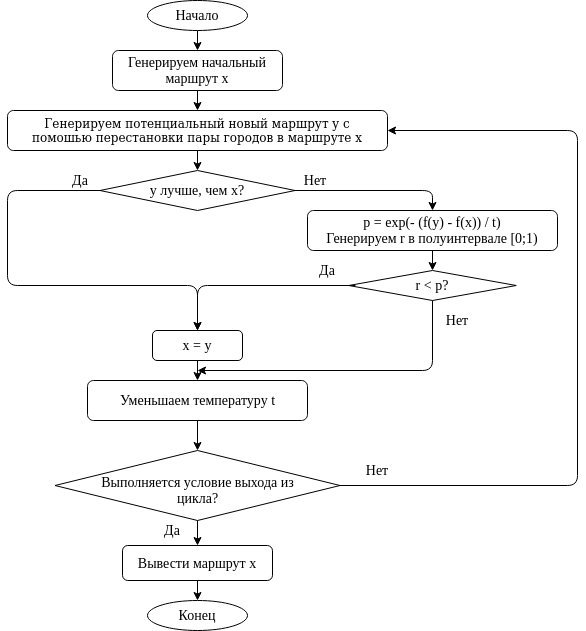
\includegraphics[scale=0.42]{Untitled_Diagram}
		\caption{Блок-схема алгоритма имитации отжига}
		\label{fig1}
	\end{center}
\end{figure}

%__________________________________________________________________________________
\subsection{Особенности реализации на языке С++}
Граф представим как матрицу смежности \texttt{std::vector<vector<double{>}{>} matrix}. Начальную температуру зададим как максимальное значение \texttt{double}. Рассмотрим особенности реализации:
\begin{itemize}
	\item Начальную перестановку получаем заполнением \texttt{std::vector<int> vertexes} числами от 0 включительно до размера матрицы смежности не включительно. Далее перемешаем элементы контейнера с помошью \linebreak \texttt{std::shuffle(vertexes.begin(), vertexes.end(), hashFunction())}.
	\item \texttt{GetWeight(vertexes, matrix)} --- это функция для подсчета суммарной длины маршрута. Суммирует вес ребер для перестановки vertexes и возвращает его.
	\item \texttt{FlipVertex(vertexes, firstN, secondN)} --- данная функция инвертирует перестановку vertexes с элемента firstN по элемент secondN.
	\item \texttt{GetVertexes(vertexes, matrix)} --- данная функция возвращает новый маршрут. Внутри нее вызывается функция \texttt{FlipVertex(vertexes, firstN, secondN)}, где \texttt{$0$ $\leq$ firstN $<$ secondN $<$ vertexes.size()} и эти числа являются случайными.
	\item \texttt{GetProbability()} --- \looser{-0.02}{это функция, которая считает вероятность по формуле}~ \eqref{prob}.
\end{itemize}

Для уменьшения вероятности ошибки алгоритм запускается несколько раз и качестве ответа выбирается перестановка с наименьшим весом.

%__________________________________________________________________________________

\section{Примеры решения модельных задач} 

Приведенные ниже примеры позволяют сравнить работу двух алгоритмов на тестах с различными входными данными.

В файле с входными данными в первой строке записано количество городов \texttt{n}, и следующие \texttt{n} строк занимает матрица смежности.



\textbf{Пример 1.} 
Рассматривается тест, состоящий из 4 городов, которые необходимо обойти. Это простейший случай задачи коммивояжера.
\begin{wraptable}{r}{3.5cm}
	
	\texttt{
		Входные данные:
		\begin{tabular}{cccc}
			4 & {} & {} & {}\\
			0 & 1 & 4 & 6 \\
			1 & 0 & 5 & 2\\
			4 & 5 & 0 & 3\\
			6 & 2 & 3 & 0\\
		\end{tabular}
	}
\end{wraptable} 
На данном тесте можно проиллюстрировать формат входных и выходных данных и наглядно показать выбранный маршрут на графе.

На рис. \ref{fig1_3} изображен взвешенный граф. Синим цветом отмечен маршрут коммивоя\-жера с минимальной длиной.
		
	\begin{figure}[!h]
		\begin{center}
			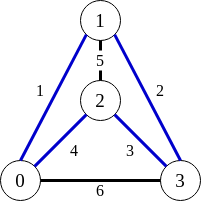
\includegraphics[scale=0.5]{Test2-1}
			\caption{Иллюстрация примера 1}
			\label{fig1_3}
		\end{center}
	\end{figure}

В таблице 1 приведено сравнение результатов работы программ, реализованных методом полного перебора и методом имитации отжига. Можно заметить, что в обоих случаях минимальный маршрут определен правильно за почти одно и то же время.

\begin{table}[h]
	\caption{Пример работы алгоритмов для 4 городов}
\begin{center}
%\bigskip
	\begin{tabular}{|p{0.21\linewidth}|p{0.15\linewidth}|p{0.15\linewidth}|p{0.19\linewidth}|p{0.14\linewidth}|} \hline
\multirow{3}*{} 
& Маршрут & Длина пути & Относительная погрешность, \% & Затраченное время, с\\ \hline
Метод перебора & 1 3 4 2 1 & 10 & 0,0 & 0,004 \\
\hline
Метод имитации отжига при \looser{-0.02}{$\texttt{coolingRate}=0.1$}, $\texttt{repeatRate}=1$ & 1 3 4 2 1 & 10 & 0,0 & 0,003 \\
\hline
\end{tabular}\\
\end{center}
\end{table}

\textbf{Пример 2.} В тесте содержится 11 городов --- это максимальное количество городов, которое может быть обработано методом полного перебора. 

В этом примере становится видно как изменяется ответ и время исполнения метода отжига при изменении параметров \texttt{coolingRate} и \texttt{repeatRate}. В таблице 2 приведены средние значения длин найденных путей для разных значений параметра \texttt{coolingRate}, они были получены на основе 1000 измерений. Можно заметить, что при увеличении \texttt{coolingRate} при маленьком \texttt{repeatRate} относительная погрешность уменьшается, а при при увеличении \texttt{repeatRate} и уменьшении \texttt{coolingRate} наблюдается обратная тенденция. Кроме того, константа \texttt{coolingRate} почти не влияет на время исполнения программы, в отличии от \texttt{repeatRate}.

\begin{table}[h]
	\caption{Пример работы алгоритмов для 11 городов}
\begin{center}
\begin{tabular}{|p{0.23\linewidth}|p{0.22\linewidth}|p{0.22\linewidth}|p{0.22\linewidth}|} \hline
		\multirow{3}*{} 
		& Средняя длина полученного пути & Относительная погрешность, \% & Затраченное время, с\\ \hline
Полный перебор                               & 0,015
 & 0   & 0,034 \\ \hline
Алгоритм имитации отжига при $\texttt{coolingRate}=0.1$, $\texttt{repeatRate}=1$ & 0,034 & 132,1 & 0,004 \\ \hline
Алгоритм имитации отжига при $\texttt{coolingRate}=0.1$, $\texttt{repeatRate}=10$ & 0,01508 & 0,5 & 0,012 \\ \hline
Алгоритм имитации отжига при $\texttt{coolingRate}=0.9$, $\texttt{repeatRate}=1$ & 0,033 & 124,7  & 0,004 \\ \hline
Алгоритм имитации отжига при $\texttt{coolingRate}=0.9$, $\texttt{repeatRate}=3$ & 0,020 & 35 & 0,006 \\ \hline
Алгоритм имитации отжига при $\texttt{coolingRate}=0.9$, $\texttt{repeatRate}=10$ & 0,0151 & 1.06 & 0,012 \\ \hline
	\end{tabular}
\end{center}
\end{table}

Также этот пример позволяет сравнить время, затраченное на решение задачи двумя разными методами. Для работы метода полного перебора требуется в несколько раз больше времени, чем для работы алгоритма имитации отжига.

\newpage
\textbf{Пример 3.} Тест состоит из 15 точек. Аналитически был получен ответ 0.01701. 

В таблице 3 приведено сравнение полученной длины пути, относительной погрешности и времени исполнения программы при разных значениях параметров \texttt{coolingRate} и \texttt{repeatRate}. Можно сделать вывод о том, что константа \texttt{coolingRate} очень слабо влияет на погрешность, однако при ее увеличении погрешность как правило снижается, а время, затраченное на исполнение программы совсем немного увеличивается. Кроме того, увеличение параметра \texttt{repeatRate} значительно улучшает точность результата, но в то же время заметно повышает время исполнения программы.

\begin{table}[h]
	\caption{Пример работы алгоритмов для 15 городов}
	\begin{center}
		\begin{tabular}{|p{0.16\linewidth}|p{0.14\linewidth}|p{0.21\linewidth}|p{0.19\linewidth}|p{0.15\linewidth}|
				p{0.22\linewidth}|}\hline
			\multirow{3}*{} 
			\texttt{coolingRate} & \texttt{repeatRate} & Средняя длина полученного пути & Относительная погрешность, \% & Затраченное время, с\\ \hline
		    0,1 & 10   & 0,04 & 135,3  & 0,018 \\ \hline
			0,1 & 20   & 0,026 & 52,9    & 0,045 \\ \hline
			0,1 & 50   & 0,019 & 8,9    & 0,076 \\ \hline
			0,1 & 100   & 0,01706 & 0,3    & 0,137 \\ \hline
			0,9 & 10    & 0,038 & 124,3 & 0,35 \\ \hline
			0,9 & 20   & 0,026 & 51,9    & 0,046 \\ \hline
			0,9 & 50   & 0,0181 & 6,4    & 0,074 \\ \hline
			0,9 & 100   & 0,01713 & 0,7    & 0,137 \\ \hline
			0,99 & 10  & 0,035 & 139,4     & 0,035 \\ \hline
			0,99 & 20   & 0,027 & 55,5    & 0,045 \\ \hline
			0,99 &  50   & 0,0184 & 8,3    & 0,075 \\ \hline
			0,99999 & 20   & 0,0255 & 50,4    & 0,044 \\ \hline
		\end{tabular}
	\end{center}
\end{table}

\newpage

%__________________________________________________________________________________

\section-{Заключение} 

Результатом выполнения практического задания стало знакомство с задачей коммивояжера и изучением метода перебора и имитации отжига.  Были написаны реализации этих методов на C++ и Wolfram Mathematica, а также выявлены их преимущества и недостатки. Метод перебора не может быть использован для вычислений маршрута коммивояжера для достаточно больших графов. Применение этого метода на практике практически не возможно, поскольку его алгоритмическая сложность $o(n!)$. Метод иметации отжига является методом приближенного вычисления и требует подбора параметров в зависимости от входных данных, однако позволяет находить решения для более сложных задач, чем метод перебора.

%__________________________________________________________________________________
% Библиотека

\newpage

\begin{thebibliography}{5}
	\bibitem{nextperm}
	next\_permutation // cppreference.\\
	URL: https://en.cppreference.com/w/cpp/algorithm/next\_permutation \\
	(дата обращения: 01.06.2022).	
	\bibitem{wiki}
	Задача о коммивояжера // Википедия. Свободная энциклопедия.\\
	URL: https://ru.wikipedia.org/wiki/Задача\_коммивояжёра\\
	(дата обращения: 01.06.2022).
	\bibitem{habr}
	Введение в оптимизацию. Имитация отжига // Хабр.\\
	URL: https://habr.com/ru/post/209610/\\
	(дата обращения: 01.06.2022).
	\bibitem{researchgateblock}
	\looser{-0.02}{
	List-Based Simulated Annealing Algorithm for Traveling Salesman Problem} // Hindawi.\\
	URL:~\looser{-0.09}{https://www.researchgate.net/figure/Flowchart-of-simulated-annealing-algorithm\_fig1\_298209081}\\
	(дата обращения: 01.06.2022).
	\bibitem{mitpaper}
	Statistical Science: Simulated Annealing / D. Bertsimas, J. Tsitsiklis // Ref. Libr. – 1993. Vol. 8. № 1. – P.10–15.
	
\end{thebibliography}

\end{document}